\documentclass[12pt]{article}
\usepackage[english]{babel}
\usepackage[utf8]{inputenc}
\usepackage{hyperref}
\usepackage{fancyhdr}
\usepackage{graphicx}
\usepackage{enumitem}
\usepackage[authoryear]{natbib}
\usepackage{eurosym}
\usepackage{geometry}
\usepackage{amsmath}
\usepackage{amssymb}
\usepackage{setspace}
\usepackage{algorithm}  % Required for algorithms
\usepackage{algpseudocode}
\usepackage{eso-pic}
\usepackage{mathtools}
\usepackage{float}
\usepackage{lipsum}
\usepackage{tocbibind}

\setstretch{2}
\geometry{
    left=1in,
    right=1in,
    top=1in,
    bottom=1in
}

\begin{document}
\title{Research-Project-Het-Patel-7972424}

\begin{titlepage}
\vspace*{\fill}
\centering
    {\LARGE\textbf{Q-Learning and Deep Q-Learning Algorithms in Reinforcement Learning}} \\
    \vspace{1 cm}
    {\LARGE Het Patel}\par
    \vspace{0.5cm}
    {\Large COMP 3190 Research Project}\par
    \vspace{0.5cm}
    {\Large Student Number: 7972424}\par
    \vspace{0.5cm}
    {\Large Date: 05 April 2024}\par
\vspace*{\fill}
\end{titlepage}

\tableofcontents

\newpage

\section{Abstract}

This research project studies the fundamentals of reinforcement learning, focusing on two distinct algorithms: Q-Learning and Deep Q-Learning. An agent learns through behavior in a given environment and receiving rewards in reinforcement learning. In the context of learning from interaction, we begin by outlining key concepts such as policies, value functions, reward signals, and actions themselves. Next, I discuss Markov Decision Processes, which are useful tools for modeling various types of learning scenarios.

The discussion then turns to Q-Learning, a technique that allows an agent to learn without requiring an environment model. It's useful for determining the appropriate course of action in various circumstances. Subsequently, we present Deep Q-Learning, which combines Q-Learning with deep learning to tackle complex problems with numerous actions and states. We go into deeply into the inner workings of these algorithms, highlighting their unique strengths and differences from one another.

\section{Introduction}

\subsection{Reinforcement Learning}

Reinforcement learning is a learning in which learner learns by interacting to the environment and observing the rewards it gets, in this a learner has to try and test multiple actions that they have and selecting the action which yielded that maximum reward by comparing different output. Sometimes, a reward can not only affect the current reward but it can affect the future rewards, and these are the two main characteristics of reinforcement learning, i.e., exploration and delayed rewards \cite{Sutton_Barto_2020}. As in reinforcement learning the problems are solved by focusing on learning by directly interacting with the environment, it make reinforcement learning different from other learning techniques like supervised and unsupervised learning. A policy, a reward signal, a value function, a model, an agent, an action and an observation are main sub element of reinforcement learning [\cite{Sutton_Barto_2020}].

\subsection{A Policy}

A policy describes all possible ways an agent can take at a given state from the environment and time [\cite{Sutton_Barto_2020}]. A policy can be a lookup table, simple function or sometimes a complex computational search process, but they are probabilities for each action [\cite{Sutton_Barto_2020}].

\subsection{A Reward Signal}

When an agent performs a action, a reward is provided to the agent from the environment and the agent's objective is to maximize that reward in long time. So, in long run there will be good events and bad events depending upon the current state, environment and action performed and the reward signal will define whether an event is good or bad. Moreover, a reward signal have other roles like changing the policy and defining goal state [\cite{Sutton_Barto_2020}].

\subsection{A Value Function}

A value function as it's name return a value associated to a state, it is the expected total amount of reward for an agent to get in future when the starting point is that state [\cite{Sutton_Barto_2020}]. A value generated from the value function for a particular state is long term expected rewards, where as a reward is the immediate thing for that state. A low reward state might have high value and vice versa [\cite{Sutton_Barto_2020}].

\subsection{An Action}

Action is the things that an agent can perform to move from one state to another, an action can be discrete or continuous. An example for discrete action is moving left, right, up or down in a game and an example for continuous action can be moving a steering wheel as it can be moved at many angles [\cite{Lapan_2020}].

\begin{figure}[H]
\centering
  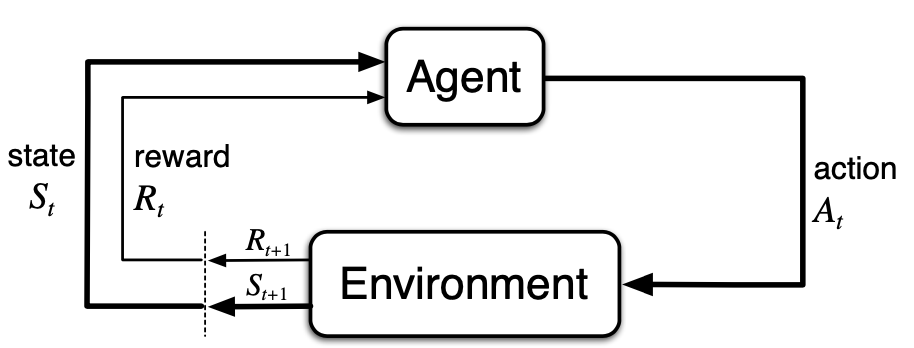
\includegraphics[width=0.5\textwidth]{images/agent-env.png}
  \caption{Agent-Environment Interaction in MDP [\cite{Sutton_Barto_2020}]}
  \label{agent-env}
\end{figure}


\section{Markov Decision Process}

The reinforcement learning can be expressed in terms of Markov Decision Process, as in reinforcement learning their are states, actions, immediate and delayed rewards [\cite{Sutton_Barto_2020}]. Markov decision process consist of a state space $\mathcal{S}$, a function $\mathcal{A}$ that provides possible actions for each state and $\mathcal{A}(x)$ is a set of every action available for state $x \in \mathcal{S}$, a transition function $\mathcal{T}$ and a reward function $\mathcal{R}$ [\cite{1989}].


\subsection{Definition of Markov Decision Process}
The agent and environment interact with each other at a sequence of discrete timestamp t = 0, 1, 2, 3, $\dots$. For each $t$ agent receives a numerical reward $R_{t+1} \in \mathcal{R}$, base on the state $S_t \in \mathcal{S}$ and action, $A_t \in \mathcal{A}$, performed, after this the the agent find himself in new state $S_{t+1} \in \mathcal{S}$. This process is continued until the agent has not reached to the goal [\cite{Sutton_Barto_2020}]. The new state $S_{t+1}$ depends upon the state at time $t$ and action performed, i.e., on $S_t$ and  $A_t$ and this relation is provided by the transition function function $\mathcal{T}$, $$\mathcal{T}(S_t, A_t) = S_{t+1}$$ The transition function has a well defined probability distribution, so the returned state from $\mathcal{T}(S_t, A_t)$ can be sampled from probability distribution over $\mathcal{S}$ [\cite{1989}]. As we are considering finite states we can express the probability of state $S_t$ getting transitioned to new state $S_{t+1}$ after performing action $A_t$ as $$P(S_{t+1} | S_t, A_t) = Pr\{\mathcal{T}(S_t, A_t) = S_{t+1}\},$$ The above equation is the definition of the probability function P [\cite{Sutton_Barto_2020}]. Lastly, the reward function is defined to return the reward $R_t$ based on the state $S_t$ and action $A_t$, $$R_t = \mathcal{R}(S_t, A_t),$$ Generally to indicate a case of fail is defined by negative reward value [\cite{1989}]. We are more interested in the expected value of the reward function rather that the actual reward function and the expected value for reward function function is defined as $$\rho(S_t, A_t) = E[R(S_t, A_t)], \text{[\cite{1989}]}$$

\subsection{The Markov Property}

The Markov property state that the transition function and reward function is only depend on the current state and the current action, it is not dependent upon any other past state and actions. This is important, as it says that only current state is needed to select which action to perform, and we do not need any past environment information [\cite{1989}]. 

\subsection{Policy}

A policy is a function that defines rule for deciding which action to perform at a given time t and at current state $S_t$, it maps from state space to the action space [\cite{1989}]. Their are 2 different policies, stationary and stochastic policies. If a policy is returning same action for each time the state is visited it is called stationary policy, whereas if the action is selected from a probability distribution over available actions for each state it is termed as stochastic probability [\cite{1989}]. For a stochastic policy $\pi$ in state $S_t$ we can define probability of next transitioned state is $S_{t+1}$ as $$Pr(S_{t+1}) = \sum_{a \in A(x)}Pr(\pi(S_t) = a)P(S_{t+1}|S_t, A_t),$$ we can simplify the expression and denote it as $P_{S_t,A_t}(\pi)$. Similarly let $T(S_t, \pi), R(S_t, \pi), \rho(S_t, \pi)$ be next state, the reward state and the expected state under policy $\pi$ in finite state $S_t$ [\cite{1989}].

\section{Q-Learning Algorithm}

Q-Learning is a model free reinforcement learning algorithm. It does not require and model that is approximation of the environment, it provides agents the capacity of learning to act optimally Markovian domain with building any maps of domain [\cite{1992}]. The path of learning is started by an agent performing an action at a particular state, calculating and storing the values required to perform next steps. In reinforcement learning an agent is given task to find a optimal policy $\pi^*$, such that it maximise \textit{the expected discounted rewards}, and it is proved with Dynamic programming that their exist at least one optimal policy $\pi^*$[\cite{1992}]. So, this algorithm computes a Q value which is the expected discounted rewards for performing an action a in a state s while following a policy $\pi$, that is why it is called Q-Learning Algorithm [\cite{1992}]. 

\subsection{Value Function}

As described earlier value function is expected value of rewards associated with a state, it does not depend on which action was taken [\cite{Sutton_Barto_2020}]. This function maps from state space to a real number, i.e., $$V:\mathcal{S} \rightarrow \mathbb{R}, \text{[\cite{Sutton_Barto_2020}]}$$ The value function for any state $x \in \mathcal{S}$ under policy $\pi$ is defined as expected rewards when starting at \textit{x} and using $\pi$ thereafter $$V_{\pi}(x) = \rho(x, \pi(x)) + \sum_{k=0}^{\infty}\gamma^kR_{t+k+1}, \text{[\cite{Sutton_Barto_2020}]}$$ Where \textit{t} is the time of the world, $\gamma$ is discount factor and $\sum_{k=0}^{\infty}\gamma^kR_{t+k+1}$ describes the expected reward of future actions $V_{\pi}$ is also called \textit{state-value function for policy } $\pi$ [\cite{Sutton_Barto_2020}].

\subsection{The Q-Value}

First consider an agent in a world at step n with actions $\mathcal{A}$, policy $\pi$, state space $\mathcal{S}$, expected reward function $\rho(x_n,a_n)$ which return expected rewards for action $a_n \in \mathcal{A}$ performed at state $x_n \in \mathcal{S}$, and transitioned state $y_n \in \mathcal{S}$ [\cite{1989}]. Then the probability of agent performing state changing to $y_n$ is given by $$P[y_n = y | x_n, a_n] = P_{x_ny}[a_n], \text{[\cite{1992}]}.$$ Now for an agent the task is find an optimal policy $\pi^*$ which maximize the value function. To do this \cite{1989} defined a value name as action-value or Q, which represents expected discounted rewards for performing an action $a_n$ at state $x_n$. Function to calculate Q Value under a policy $\pi$ maps from combination of state and action to a real number, i.e., $$Q: \mathcal{S} \times \mathcal{A} \rightarrow \mathbb{R}, \text{[\cite{1992}]}$$

The Q value for an action and state with policy $\pi$ is given by $$Q^{\pi}(x,a) = \rho(x,a) + \gamma\sum P_{xy}[\pi(x)]V^{\pi}(y), a \in \mathcal{A}, x,y \in \mathcal{S}$$

The Q value is addition of expected rewards for performing action \textit{a} from state \textit{s} and expected reward of next state following the policy $\pi$. Here $\gamma$ is discount factor [\cite{1992}].

\cite{1989} in his thesis proved using Dynamic Programming that Q-value is helpful in finding the optimal policy, and it is computationally more efficient to use Q-values in place of value functions. With Q-value it is efficient to compare 2 policy and decide which policy to use for maximizing the rewards at particular state of particular episode.

\subsection{The Algorithm}

The agent is first trained using the reward function, states and action i the environment. During training a table containing Q values of each state action pair is stored and maintained. For each action $a_n \in \mathcal{A}$ taken from a particular state $x_n \in \mathcal{S}$ a Q-value is updated if their is new policy that yields maximum expected rewards [\cite{1992}]. The Q values is updated as following

Consider that agent performed an action $a_n$, from state $s_n$, $r_n$ be immediate reward obtained and the world transitioned into state $y_n$ at step n, then the Q value is updated as:

\begin{align*}
    Q_n(x, a) = \begin{cases}
                (1 - \alpha_n) Q_{n-1}(x,a) + \alpha_n[r_n + \gamma_n V_{n-1}(y_n)], & \text{if } x = x_n \text{ and } a = a_n \\
                Q_{n-1}(x,a), & \text{otherwise}
            \end{cases}
\end{align*}

The above definition is derived using Bellman's equation, where $V_{n-1} = \underset{\text{b}}{\text{max}}\{Q_{n-1}(y,b)\},$ maximum rewards that can be obtained from next state. $\gamma \text{ is discount factor, } \alpha$  is learning rate [\cite{1992}].

The Q-Learning algorithm tries to estimate the q value for an optimal policy and Q-Learning is a primitive learning [\cite{1992}]. A \textit{primitive learning } is a learning in which agent does not have any details related to transition and rewards model. The recursion model is for learning is called \textit{One step Q-Learning}, in this process the Q value for corresponding state and action is updated every time that particular pair of state and action is taken place and rest of the combinations are left unchanged. An agent is free to choose any action it wants as eventually it is value iteration method and is one of conventional algorithm from dynamic programming. Moreover, for agent to find the optimal value function the agent should explore all of the states  [\cite{1989}].

\subsection{The Training Process}

One can choose how many times they want to train the agents in the environment by defining number of episodes. At the start of the training process, Q value table is initialized to zero and then it is updated as the algorithm moves forward. Random sampling from the distribution of the action space $\mathcal{A}$ and state space $\mathcal{S}$ is use to choose actions and starting point of the training process [\cite{Szepesvari_2022}]. Once the Q table is finalized and the agent is performing real task in the environment, the optimal policy to choose the action is defined as $$\pi^*(x) = \underset{a}{max}\{Q(x,a)\} \text{, where } x \in \mathcal{S} \text{ and } a \in \mathcal{A}, [\cite{1989}]$$ 

Below is the algorithm for the \textit{off policy} training process for an agent using Q-learning from \cite{Sutton_Barto_2020}

\begin{algorithm}
\caption{Q-Learning for estimation $\pi \approx \pi^*$}
\label{alg:q_learning}
\begin{algorithmic}[1]
\State Algorithm parameters: step size $\alpha \in (0, 1]$, small $\epsilon$ \> 0, number of episodes \textit{n}
\State Initialize \textit{Q(s,a)} = 0, $\forall s \in \mathcal{S}, a \in \mathcal{A}(s)$, except goal state $s_g$
\State
\State Loop for each episode:
    \State \hspace{\algorithmicindent} Initialize \textit{x}
    \State \hspace{\algorithmicindent} Loop for each step of episode:
        \State \hspace{\algorithmicindent} \hspace{\algorithmicindent} Choose action \textit{a} from \textit{x} using policy derived from \textit{Q}, (e.g., $\epsilon$-greedy)
        \State \hspace{\algorithmicindent} \hspace{\algorithmicindent} Take action \textit{a} and observe \textit{r} and \textit{y}
        \State \hspace{\algorithmicindent} \hspace{\algorithmicindent} $Q_n(x, a) = (1 - \alpha) Q_{n-1}(x,a) + \alpha_n[r + \gamma_n V_{n-1}(y)]$
        \State \hspace{\algorithmicindent} \hspace{\algorithmicindent} \textit{x} $\leftarrow$ \textit{y}
    \State \hspace{\algorithmicindent} Until $x$ is not $s_g$ 
\end{algorithmic}
\end{algorithm}

\section{Deep Q-Learning Algorithm}

Before going into Deep Q-Learning let use understand few concepts that will help understanding Deep-Q Learning better. Deep Q-Learning is a way of learning that comes under the concept of Deep Reinforcement learning and when Deep Learning and Reinforcement learning are applied together it is called Deep Reinforcement Learning [\cite{yuxi}]. Deep Q-Learning was first introduced by \cite{mnih} at DeepMind, in that they let the agent which was trained using Deep Q-Learning play the Atari game and achieved human level control. This algorithm is also use in various place for example, in image enhancement, building chat bot in natural language processing [\cite{yuxi}]. Deep Q-Learning is part of Deep Reinforcement Learning, and Deep RL is an implementation of combination of Deep Learning with Reinforcement Learning [\cite{Zou_Han_So_2008}]

\begin{figure}[H]
\centering
  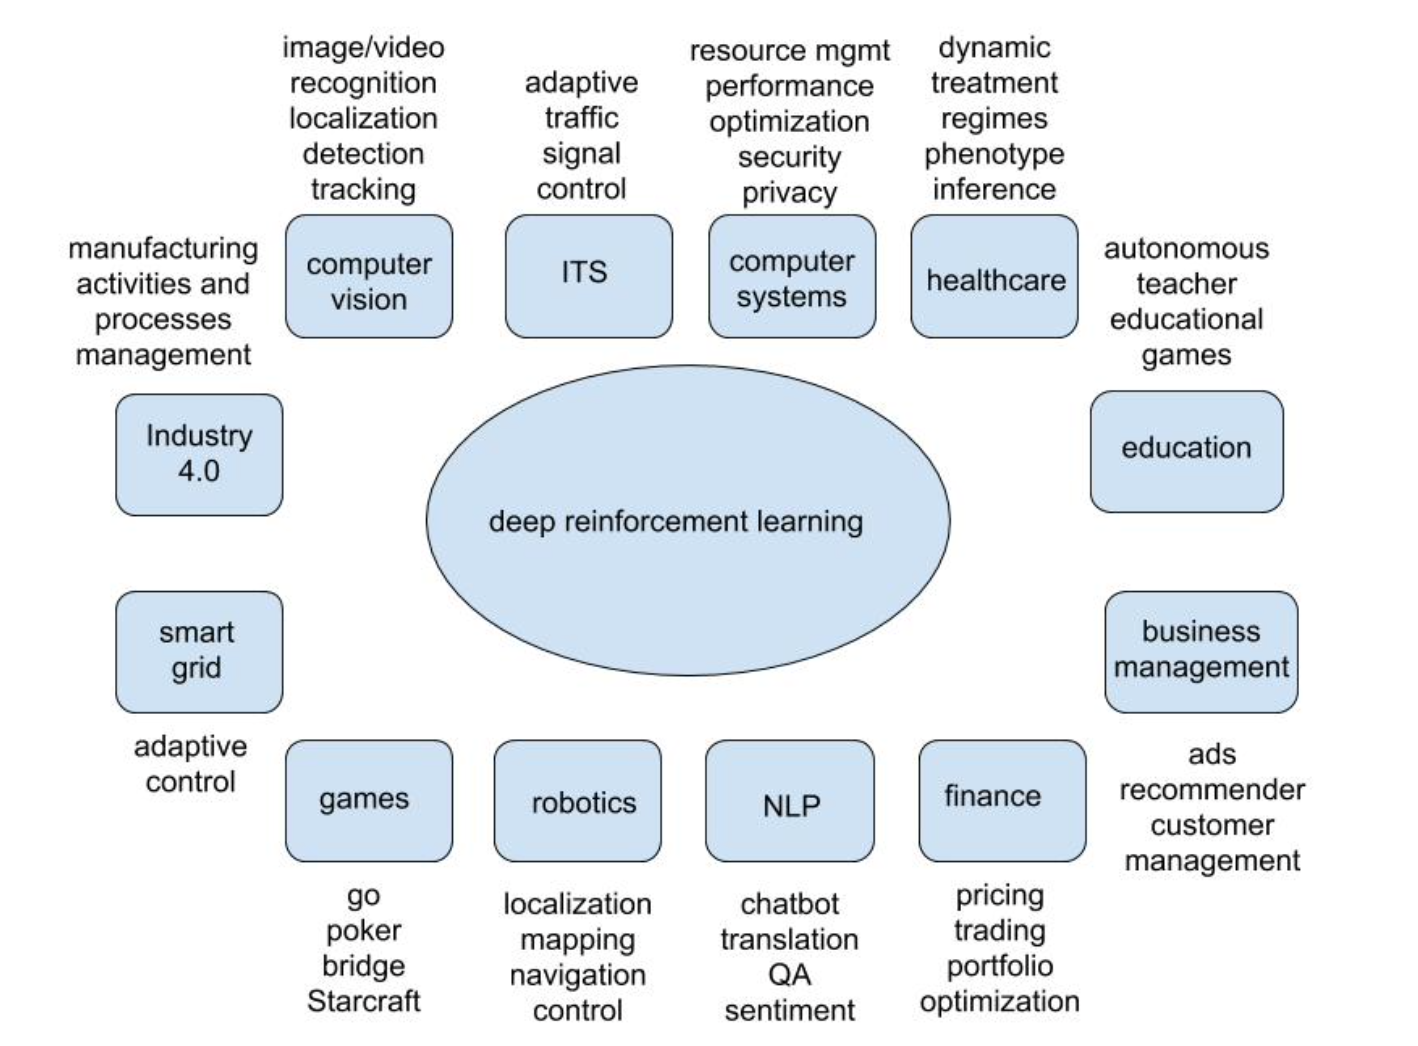
\includegraphics[width=0.5\textwidth]{images/drl-imp.png}
  \caption{Deep Reinforcement Learning Applications [\cite{yuxi}]}
  \label{drl-imp}
\end{figure}

\subsection{Deep Learning}

Deep Learning is a branch of Machine which uses \textit{Artificial Neural Network} (ANN) in practice to run algorithms and provide the solution to the given problem [\cite{laura}]. Artificial Neural Network mimics the biological neurons present in the human body [\cite{laura}]. A ANN is connection of nodes and it has 3 main components,  which are node character, network topology and learning rules (Hao Dong).

Node structure and connectivity are determined by network topology, and weight initialization and modification are governed by learning rules. Each component will be thoroughly explained in the sections that follow [\cite{Zou_Han_So_2008}]. An ANN have an input layer, an output layer and there are connection layer between the input and output layer called hidden layer, moreover, A layer is linear array of nodes [\cite{Zou_Han_So_2008}]. Each node get input from multiple other nodes and the associated weight is calculated and if the weight is greater than threshold value then that node is activated and pass the signal forward using the transfer function [\cite{Zou_Han_So_2008}].

The models that uses these ANN in more complex manner are known as Deep Learning models or algorithms. Sometimes, the complex Artificial Neural Network are also referred as Deep Neural Network in Deep Learning (Hao Dong).


\subsection{DQN}

This algorithm uses Deep Neural Network to compute the Q-values of each available action for each state that is being visited, these network are called Deep Q Network, or DQN. This is an \textit{off-policy} algorithm, meaning it does not need any information from the world other than the rewards, current and next state [\cite{laura}].

Furthermore, DQN are made upon 2 important concepts out of which first is \textit{Replay Buffer} and second is \textit{Target Network}. Using both approach in DQN improves it's stability (Hao Dong).

\begin{figure}[H]
\centering
  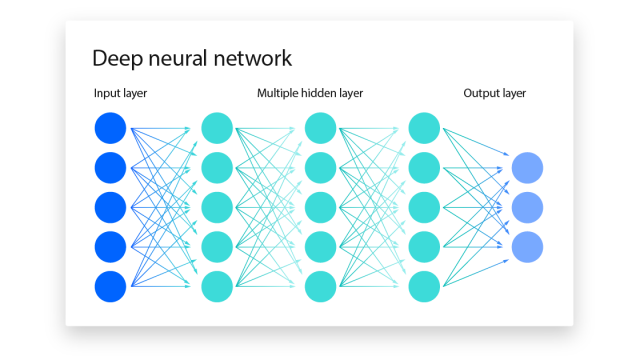
\includegraphics[width=0.5\textwidth]{images/dnn.png}
  \caption{Deep Neural Network [\cite{ibm}]}
  \label{dnn}
\end{figure}

\subsection{Replay Buffer}

At each step $n$ the DQN stores the $k$ most resent experiences of the agent, an experience is the current state, next state, action performed and reward received at step $n$ (Hao Dong). This replay buffer is also called \textit{experience replay}, and the value of $k$ generally from 10,000 to 1,000,000. Once the memory is full of a particular step the oldest experience is drooped and the new experience is add into the memory [\cite{laura}].

\subsection{Target Network}

In DQN there are 2 same Deep Neural Network, first network is used to calculate the Q-value and the second network the Target Network[\cite{jia}]. At the start of the process both of the tables reinitialized to the same values and during the training of the agent the first network is update with Q-values, after the $N$ iterations the \textit{Target Network} will get initialized with the all of the value from the main network, it can be done either by \textit{hard update} copying all of the value or by copying exponentially decaying average which is \textit{soft update} [\cite{zhang}]. $Q(s,a|\theta_i)$ represent the output of the Q-value network with $\theta$ is the weight of neural network, at iteration \textit{i} and this is use to evaluate the value function of the current state action pair, $Q(s,a; \theta^-_i)$ represent the output of the target value network [\cite{jia}]. Now at last, the Q-value function is updated by the following loss function $$L(\theta_i) = \mathbb{E}_{s,a,r,s'}[(y_i - Q(s,a|\theta_i))^2], \text{where } y_i = r + \gamma max_{b}Q(s',b; \theta^-_i)$$ $y_i$ is the approximate target value calculated using weight $\theta_i^-$ from previous iteration. The above loss function is derived by minimizing the mean square error between current value network and the target Q-value in the Bellman equation [\cite{mnih}]. Talking the derivation of the Loss function with respect to weight we obtain the following gradient $$+\prescript{}{\theta_i}{L}(\theta_i) = \mathbb{E}_{s,a,r,s'}[(r + max_{b}Q(s',b;\theta^-_i) - Q(s,a;\theta_i)) + \prescript{}{\theta_i}{Q(s,a;\theta_i)}], [\cite{mnih}]$$

\subsection{The Process of Training DQN}

The training algorithm begins by initializing the replay memory $D$ with a capacity of $k$ transitions. This memory stores past experiences in the form of transitions $(s, a, r, s')$, where $s$ is the state, $a$ is the action, $r$ is the reward, and $s'$ is the next state. The action-value function $Q$ is initialized with random weights $\theta$, and a target action-value function $Q'$ is also initialized with weights $\theta^-$ initially set to $\theta$ [\cite{mnih}].

During training episodes, the agent interacts with the environment. At each time step $t$, it selects an action $a_t$ based on an exploration-exploitation strategy, such as epsilon-greedy where with probability $\epsilon$ a random action is selected, otherwise, the action with the maximum Q-value is chosen using the current weights $\theta$ of the action-value function $Q$. The agent then executes the action $a_t$, observes the reward $r_t$, and transitions to the next state $s_{t+1}$. These experiences are stored in the replay memory $D$ [\cite{mnih}].

Periodically, the agent samples a minibatch of transitions from $D$ to update the weights $\theta$ of the action-value function $Q$ using gradient descent. This step involves minimizing the loss function $L(\theta_i)$, which measures the squared difference between the predicted Q-value $Q(s, a|\theta_i)$ and the target Q-value $y_i$, where $y_i$ is calculated based on the Bellman equation using the target action-value function $\hat{Q}$ [\cite{mnih}]. 

Additionally, every $k$ steps, the target action-value function $\hat{Q}$ is updated by copying the weights from $Q$. This helps stabilize the learning process by providing a target that is less volatile compared to the constantly changing Q-values during training [\cite{mnih}].

Overall, the algorithm combines deep Q-learning with experience replay to improve the learning efficiency and stability of training deep Q-networks in reinforcement learning tasks, where the agent learns to make optimal decisions in complex environments [\cite{mnih}].
\newpage
Below is the algorithm for training the agent for deep q-network given in \cite{mnih}

\begin{algorithm}
\caption{Deep Q-learning with Experience Replay}
\label{alg:dqn_experience_replay}
\begin{algorithmic}[1]
\State Initialize replay memory $D$ to capacity $k$
\State Initialize action-value function $Q$ with random weights $\theta$
\State Initialize target action-value function $Q^{\prime}$ with weights $\theta^- = \theta$
\For{$episode = 1$ to $M$}
    
    \For{$t = 1$ to $T$}
        \State With probability $\epsilon$, select a random action $a_t$; \State otherwise, select $a_t = \text{argmax}_a Q(s_t, a; \theta)$
        \State Execute action $a_t$ in emulator, observe reward $r_t$
        \State Store transition $(s_t, a_t, r_t, s_{t+1})$ in $D$ 
        \State Sample random minibatch of transitions $(s_j, a_j, r_t, s_{j+1})$ from $D$ 
        \State if episode terminates at step $j + 1$
        \State \hspace{\algorithmicindent} Set $y_i$ = $r_j$
        \State \hspace{\algorithmicindent} otherwise Set $y_i$ = $r_j + \gamma\text{max}_{a'}\hat{Q}(s_{j+1},a';\theta^-)$
        \State Perform gradient descent step w.r.t network parameters $\theta$
        \State Every \textit{k} steps reset $\hat{Q} = Q$
    \EndFor
\EndFor
\end{algorithmic}
\end{algorithm}

Once the DQN is finalized and the agent is performing real task in the environment, the optimal policy to choose the action can be defined in the same way as in the Q-learning $$\pi^*(x) = \underset{a}{max}\{Q(x,a)\} \text{, where } x \in \mathcal{S} \text{ and } a \in \mathcal{A}$$

\section{Comparing the Two Algorithms}

Both Q-Learning and Deep Q-Learning algorithms are \textit{off-policy}, and \textit{off-policy} algorithm means that the Q-value of the next transitioned state does not depend on the policy used to gather experience [\cite{laura}]. Both have its own advantages and disadvantages and can best best if implemented in certain environments.

Based on the information I gathered, Q-Learning can be used to in environments in which the state space set and available action set are finite as well as low in carnality. The reason being Q-Learning uses value iteration and to get an optimal policy, it should visit every $|\mathcal{S}| \times |\mathcal{A}|$ action pair and this number can be very large even for some finite state and action set like for Atari game. So to same some of the computational time it is better to go with Q-Learning with relatively low state and action set.

While on the other hand, Deep Q-Learning can handle relative large but also finite state and action space quite well compared to Q-Learning as it is using Deep Neural Network and it is estimating the optimal Q-value function for a state-action pair by using a loss function and gradient descent, which is implemented by target network. It also consider the past experience from the replay buffer to make prediction more precise. But this comes at the cost of memory, because we need relatively large amount of memory to store past experience, both of the DQNs one for q-value and second for target values, compare to just a table with $|\mathcal{S}|$ rows and $|\mathcal{A}|$ columns in Q-learning.

\section{Conclusion}

In conclusion, this research gives a detailed look at Q-Learning and Deep Q-Learning in reinforcement learning. Q-Learning works well for smaller and simpler problems where it keeps adjusting its strategies to find the best ones. On the other hand, Deep Q-Learning uses advanced techniques like deep neural networks to handle bigger and more complicated challenges effectively. Comparing them, Q-Learning is easier to understand but might not work as well for really big problems. Deep Q-Learning can handle big problems but needs more computer power and memory. Both methods have their strengths and can be useful depending on the situation and how hard the problem is. Overall, this research helps us understand these learning methods better and how they can be used in different areas.

\newpage
\bibliographystyle{dinat}
\bibliography{ref}
\addcontentsline{toc}{section}{References}
\end{document}
